\documentclass{article} % For LaTeX2e
\usepackage{nips12submit_e,times}
\usepackage{amsmath}
\usepackage{graphicx}
\usepackage{caption}
\usepackage{subcaption}
\usepackage[top=1.0in, bottom=1.0in, left=1.0in, right=1.0in]{geometry}

%\renewcommand\refname{Papers To Read}
\title{Semantic Segmentation Using Hybrid Markov Logic Networks}

\author{
Aravindh Mahendran \\
\texttt{amahend1@andrew.cmu.edu} \\ 
\And
Nitish Thatte \\
\texttt{nitisht@andrew.cmu.edu} \\
\AND
Adwait Gandhe \\
\texttt{agandhe@andrew.cmu.edu} \\
}

\newcommand{\fix}{\marginpar{FIX}}
\newcommand{\new}{\marginpar{NEW}}

\nipsfinalcopy

%------------------------------------------------------------------------------------------

\begin{document}
\maketitle

\begin{abstract}
Semantic segmentation is the process of partitioning pixels in an image into categories and is a high level vision problem. Increasing the number of labels increases the complexity of the problem further. Markov Logic Networks (MLN) allow us to handle the uncertainty and complexity in a single framework, whereas Hybrid Markov Logic Networks (HMLN) are an extension of the MLNs that allow the continuous properties and functions over those properties as features.  In this paper, we propose a method for semantic segmentation using Hybrid Markov Logic Networks, which integrate logical and statistical learning. We test our results on the CAMVID dataset (Cambridge-Driving Labeled Video Database) and compare them against the results obtained using Naive Bayes method. 
\end{abstract}


\section{Introduction}
\label{sec:Intro}
Semantic segmentation is the process of classification of an image at the pixel level, which involves assigning a class label to each pixel of the image. Recognition of such semantic labels is an important problem in computer vision for understanding the underlying information in an image. While classical segmentation techniques group together the pixels based on low level features, semantic segmentation adopts a supervised learning approach. Several techniques proposed for semantic segmentation make use of low level features and a learning framework to combine them with their higher level labels.   \cite{Leibe04combinedobject} is one of the first approaches for simultaneous object segmentation and recognition that uses an Implicit Shape Model, which integrates both capabilities into a common probabilistic framework. \cite{cao:spatially} proposes a generative model based on the bag of words representation for such simultaneous recognition and segmentation. \cite{Borenstein04combiningtop} discusses how to combine bottom-up and top-down approaches into a single figure ground segmentation process that draws merits from both the approaches. \cite{Russell:2006:UMS:1153171.1153637} uses topic discovery models to learn the objects and choose the right segmentation. \cite{lin07multiple} propose a similar approach using bag of keypoints model integrated over mean-shift patches. \cite{conf/bmvc/CsurkaP08} propose a method based on some of these approaches for scoring low-level patches according to their class relevance and propagating these posterior probabilities to pixels. Contrary to these methods, certain approaches use random fields to incorporate local cues and impart global control without implementing low level segmentation. \cite{Kumar:2005:OC:1068507.1068889} propose a Bayesian method for combining up-down and bottom-up cues. \cite{Richard04multiscaleconditional} and \cite{Kumar:2005:HFF:1097115.1097790} use conditional random fields for this purpose. \cite{Shotton06textonboost:joint} discusses an approach to learning a discriminative model of object classes incorporating appearance, shape and context information efficiently. 

The motivation behind this work is the second of these approaches that uses a random field for using local cues and learning the labels globally. \cite{Domingos06unifyinglogical} discusses how Markov Logic combines the complexity and uncertainty by attaching weights to first-order formulas and viewing them as templates for features of Markov Networks. Markov Logic Networks (MLNs) \cite{Richardson06markovlogic} combine first-order logic and Markov networks and allow us to handle complexity and uncertainty in one consistent framework. Hybrid Markov Logic Networks (HMLNs)\cite{Wang_hybridmarkov} also allow for continuous properties to appear as features. 

This paper is structured as follows: Section \ref{sec:Related} discusses the related work in semantic segmentation and Hybrid Markov Logic Networks. In section \ref{sec:Attempt}, we discuss attempted methods that we have proposed for the semantic segmentation. The experiments conducted and the results obtained are presented in section \ref{sec:Exp}. Section \ref{sec:New} presents our approaches for the second half of the semester. We summarize our conclusions in section \ref{sec:Conclusion}. And finally section \ref{sec:Plan} outlines what we will accomplish in the second half of the semester.

%------------------------------------------------------------------------------------------

\section{Related Work}
\label{sec:Related}
\subsection{sec:Geo}

A recent approach for semantic image segmentation is 
%------------------------------------------------------------------------------------------

\section{Attempted Methods}
\label{sec:Attempt}
%------------------------------------------------------------------------------------------
\subsection{Label Propagation}
\label{sec:AttemptLabProp}

	In the section \ref{sec:Geo}, we discussed a method of propagating labels on a graph of connected superpixels based on a learned label transfer confidence function. This method introduced us to two ideas: propagating labels rather than directly minimizing a cost function to arrive at a segmentation and working with graphs of related superpixels. Building on these ideas, one approach we decided to pursue is to learn the weights for a hybrid Markov logic network in order to refine a prior expected segmentation obtained from a baseline algorithm through maximum a posteriori estimation. The method incorporates an undirected graph of connected superpixels that expresses where labels can propagate.

Examples of numeric terms and predicates in this Markov logic network are:

\begin{align*}
	&featureDistance(s_i,s_j)\\
	&isLabel(s_i,l_k) \\
	&isNeighbor(s_i,s_j)
\end{align*}

Where $s_i$ is the $i^\textrm{th}$ superpixel in an image and $l_k$ is the $k^\textrm{th}$ label. $featureDistance()$ is a numeric term that returns the computed distance between two image feature vectors via a distance metric such as euclidean or cosine distance. $isLabel()$ returns 1 if superpixel $s_i$ has label $l_j$ and 0 otherwise, and $isNeighbor$ returns 1 if its arguments are the neighbors and 0 otherwise. 

An example of a formula in this hybrid Markov logic network that use these predicates and numeric terms are :

\begin{equation*}
	[isNeighbor(s_i,s_j) \Rightarrow (isLabel(s_i,l_k) \Leftrightarrow isLabel(s_k,l_m))]*(featureDistance(s_i, s_k, f_m))
\end{equation*}

This formula encodes the following two beliefs about how and why labels can propagate in the image.

\begin{enumerate}
\item
	Superpixels with similar feature vectors should have the same label.
\item
	Superpixels that are connected by an edge (are neighbors) should have the same label.
\end{enumerate}

A brute-force approach to this problem would be to allow every super pixel to transfer its label to every other superpixel. This would result in a complete graph, where there is an edge between every two distinct nodes. Such a graph would allow superpixel labels to be learned from a more global context in the image. However, there would be an immense number of formulas for which to learn weights, making finding the solution computationally intractable. 

In contrast, a simple approach, which has been attempted in the past, \cite{} %insert reference%
is to connect nodes that are directly share borders. Consequently, the graph would very few edges, greatly reducing the number of required learned weights and simplifying the learning problem. This approach, however, would only use local context for label propagation.

Therefore, we propose to take a middle ground approach that will produce densely connected superpixels where relations are expected to be strong, and fewer edges across boundaries expected to not share labels. In order build this superpixel graph, we take two levels of superpixel segmentations: A coarse level, which we will henceforth refer to as supersuperpixels, and a fine level, termed superpixels. All superpixels within a supersuperpixel are connected allowing for contextual information to be shared within a region. Additionally superpixels that share a boundary between two supersuperpixels are connected allowing for labels to propagate across supersuperpixels while acknowledging that label transfer across supersuperpixels is less probable than within a supersuperpixel.

\section{Experiment}
\label{sec:Exp}
\begin{figure}
	\centering
	\begin{subfigure}[c]{\textwidth}
		\centering
		\begin{subfigure}[c]{0.195\textwidth}
			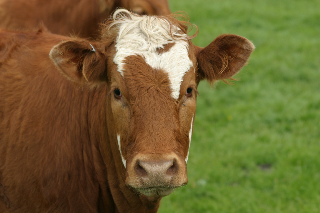
\includegraphics[width = \textwidth]{./img/1_22_s.png}
			\label{fig:1_22_s}
		\end{subfigure}
		\begin{subfigure}[c]{0.195\textwidth}
			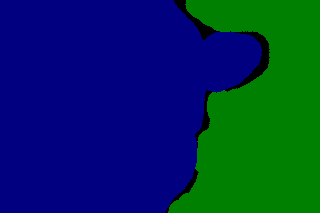
\includegraphics[width = \textwidth]{./img/1_22_s_GT.png}
			\label{fig:1_22_s_lab}
		\end{subfigure}
		\begin{subfigure}[c]{0.195\textwidth}
			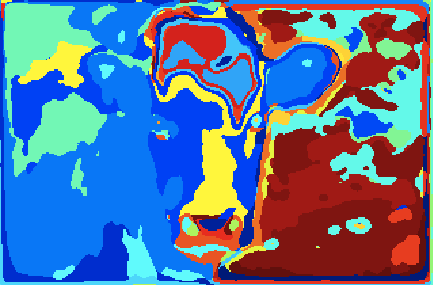
\includegraphics[width = \textwidth]{./img/1_22_s_map.png}
			\label{fig:1_22_s_map}
		\end{subfigure}
		\begin{subfigure}[]{0.195\textwidth}
			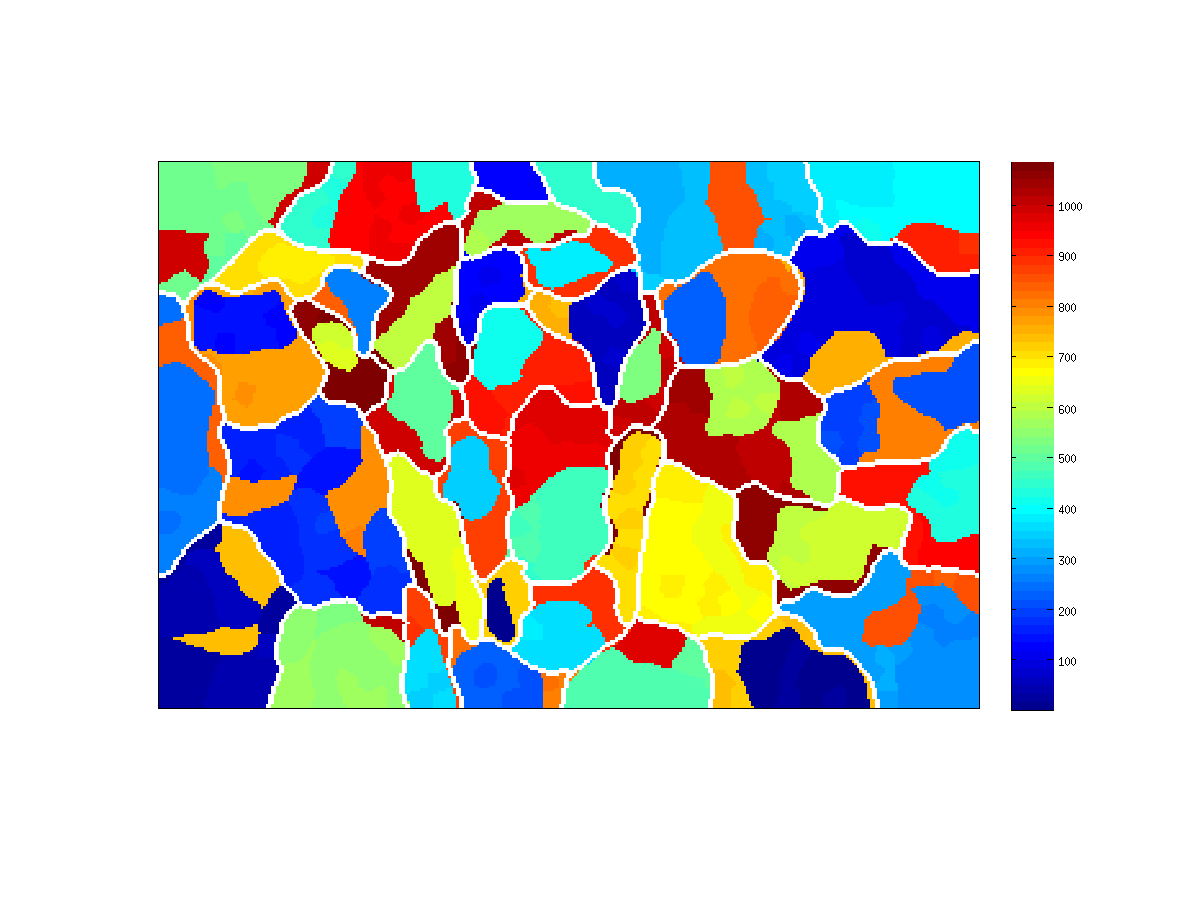
\includegraphics[width = \textwidth]{./img/su1_22_s.pdf}
			\label{fig:1_22_s_su}
		\end{subfigure}
		\begin{subfigure}[c]{0.195\textwidth}
			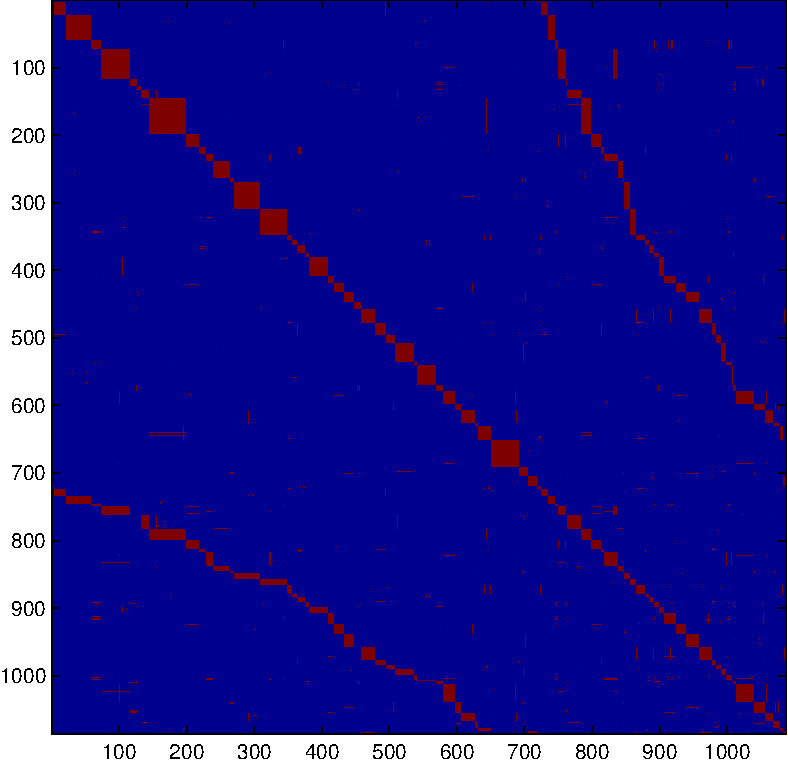
\includegraphics[width = \textwidth]{./img/adj1_22_s.pdf}
			\label{fig1_22_s_adj}
		\end{subfigure}
	\end{subfigure}

	\begin{subfigure}[c]{\textwidth}
		\centering
		\begin{subfigure}[c]{0.195\textwidth}
			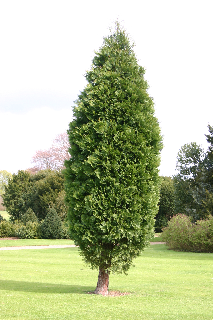
\includegraphics[width = \textwidth]{./img/2_21_s.png}
			\label{fig:2_21_s}
		\end{subfigure}
		\begin{subfigure}[c]{0.195\textwidth}
			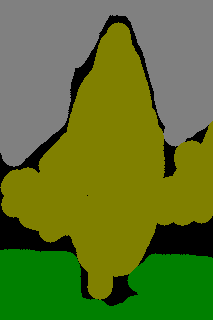
\includegraphics[width = \textwidth]{./img/2_21_s_GT.png}
			\label{fig:2_21_s_lab}
		\end{subfigure}
		\begin{subfigure}[c]{0.195\textwidth}
			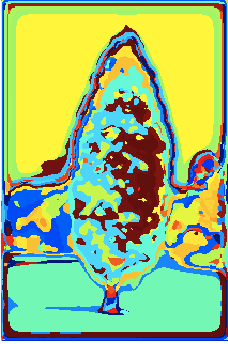
\includegraphics[width = \textwidth]{./img/2_21_s_map.png}
			\label{fig:2_21_s_map}
		\end{subfigure}
		\begin{subfigure}[]{0.195\textwidth}
			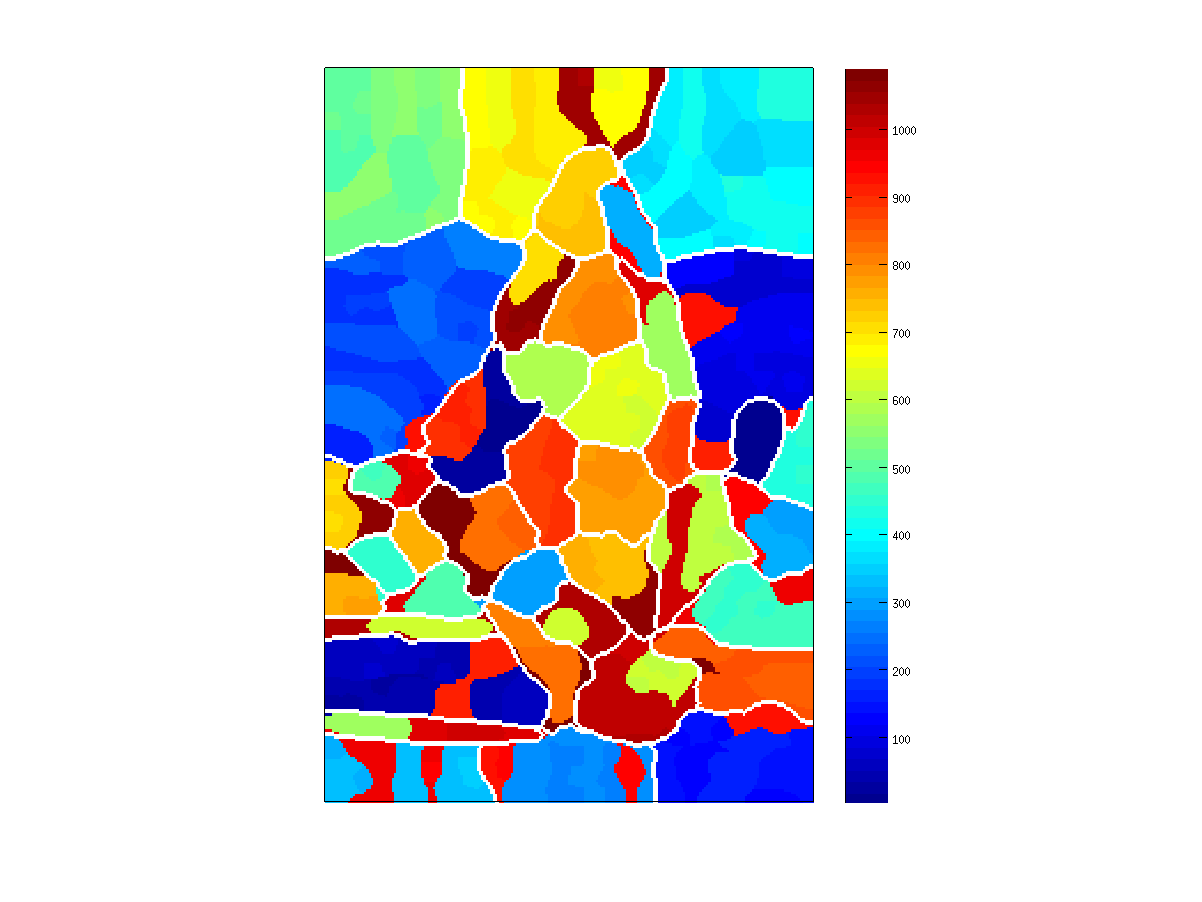
\includegraphics[width = \textwidth]{./img/su2_21_s.pdf}
			\label{fig:2_21_s_su}
		\end{subfigure}
		\begin{subfigure}[c]{0.195\textwidth}
			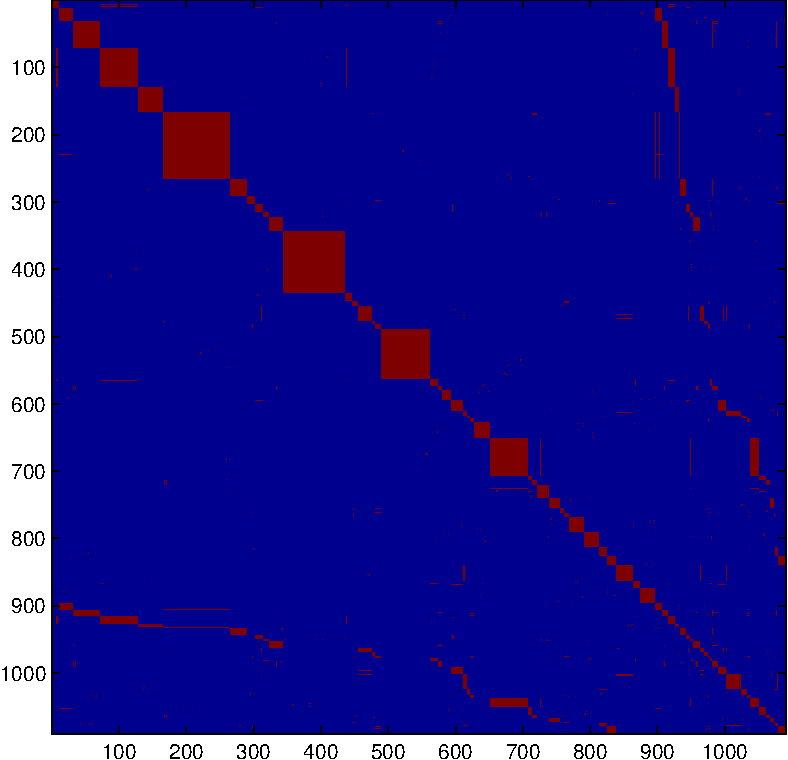
\includegraphics[width = \textwidth]{./img/adj2_21_s.pdf}
			\label{fig2_21_s_adj}
		\end{subfigure}
	\end{subfigure}

	\begin{subfigure}[c]{\textwidth}
		\centering
		\begin{subfigure}[c]{0.195\textwidth}
			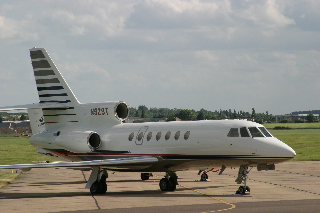
\includegraphics[width = \textwidth]{./img/4_1_s.png}
			\label{fig:4_1_s}
		\end{subfigure}
		\begin{subfigure}[c]{0.195\textwidth}
			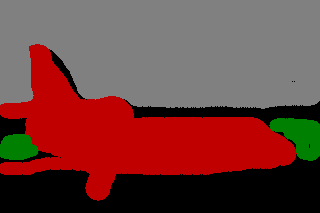
\includegraphics[width = \textwidth]{./img/4_1_s_GT.png}
			\label{fig:4_1_s_lab}
		\end{subfigure}
		\begin{subfigure}[c]{0.195\textwidth}
			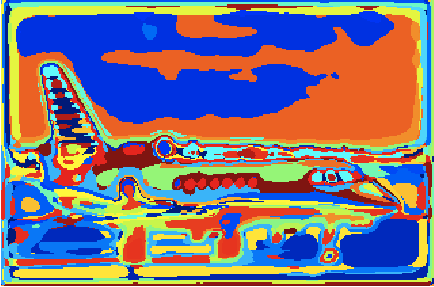
\includegraphics[width = \textwidth]{./img/4_1_s_map.png}
			\label{fig:4_1_s_map}
		\end{subfigure}
		\begin{subfigure}[]{0.195\textwidth}
			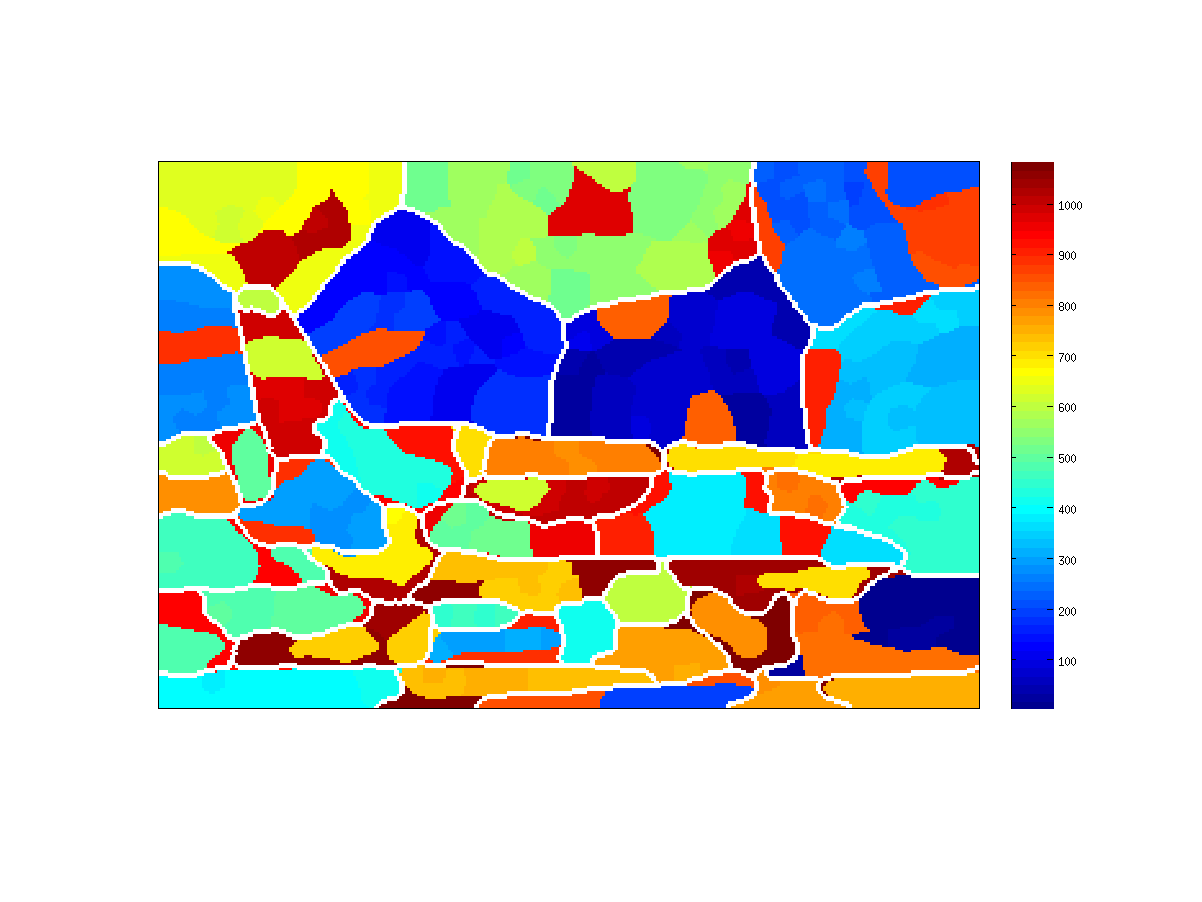
\includegraphics[width = \textwidth]{./img/su4_1_s.pdf}
			\label{fig:4_1_s_su}
		\end{subfigure}
		\begin{subfigure}[c]{0.195\textwidth}
			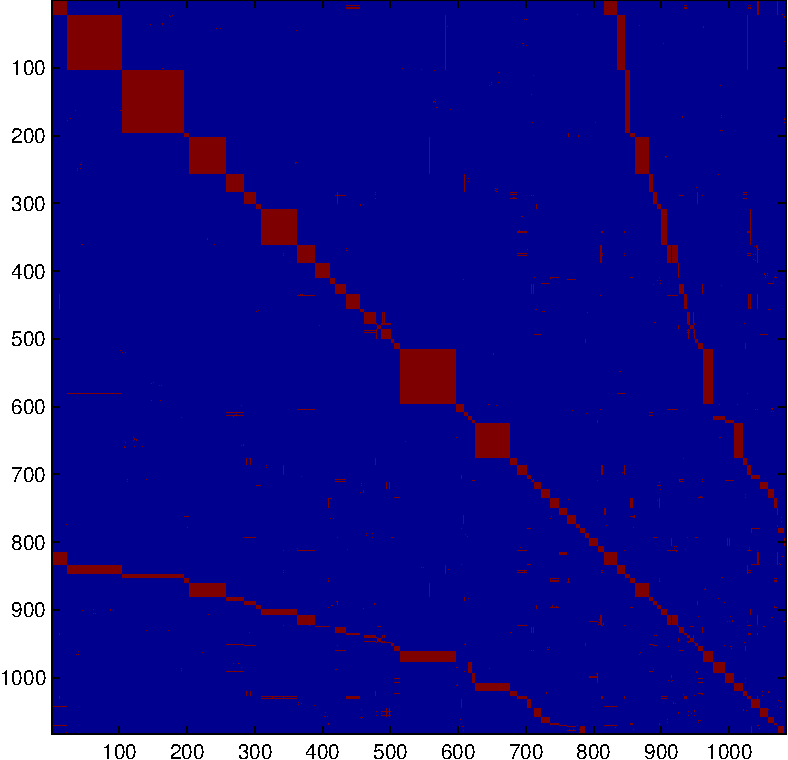
\includegraphics[width = \textwidth]{./img/adj4_1_s.pdf}
			\label{fig4_1_s_adj}
		\end{subfigure}
	\end{subfigure}

	\begin{subfigure}[c]{\textwidth}
		\centering
		\begin{subfigure}[c]{0.195\textwidth}
			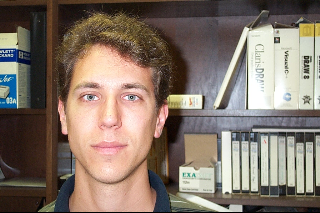
\includegraphics[width = \textwidth]{./img/6_3_s.png}
			\label{fig:6_3_s}
		\end{subfigure}
		\begin{subfigure}[c]{0.195\textwidth}
			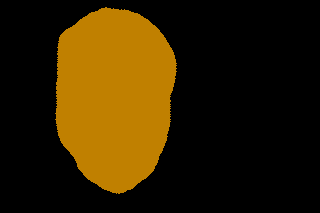
\includegraphics[width = \textwidth]{./img/6_3_s_GT.png}
			\label{fig:6_3_s_lab}
		\end{subfigure}
		\begin{subfigure}[c]{0.195\textwidth}
			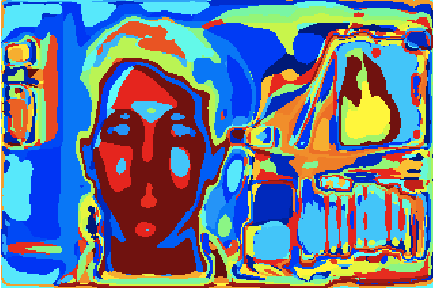
\includegraphics[width = \textwidth]{./img/6_3_s_map.png}
			\label{fig:6_3_s_map}
		\end{subfigure}
		\begin{subfigure}[]{0.195\textwidth}
			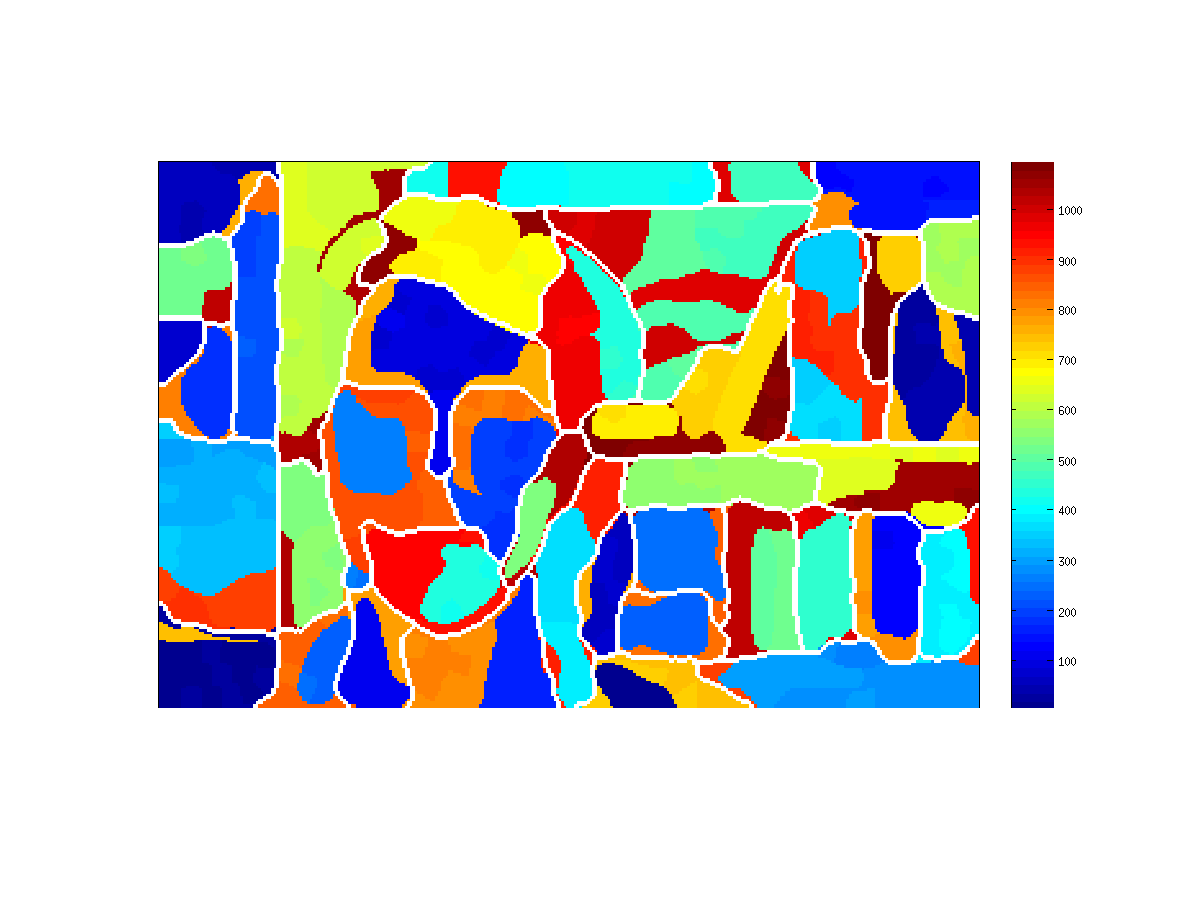
\includegraphics[width = \textwidth]{./img/su6_3_s.pdf}
			\label{fig:6_3_s_su}
		\end{subfigure}
		\begin{subfigure}[c]{0.195\textwidth}
			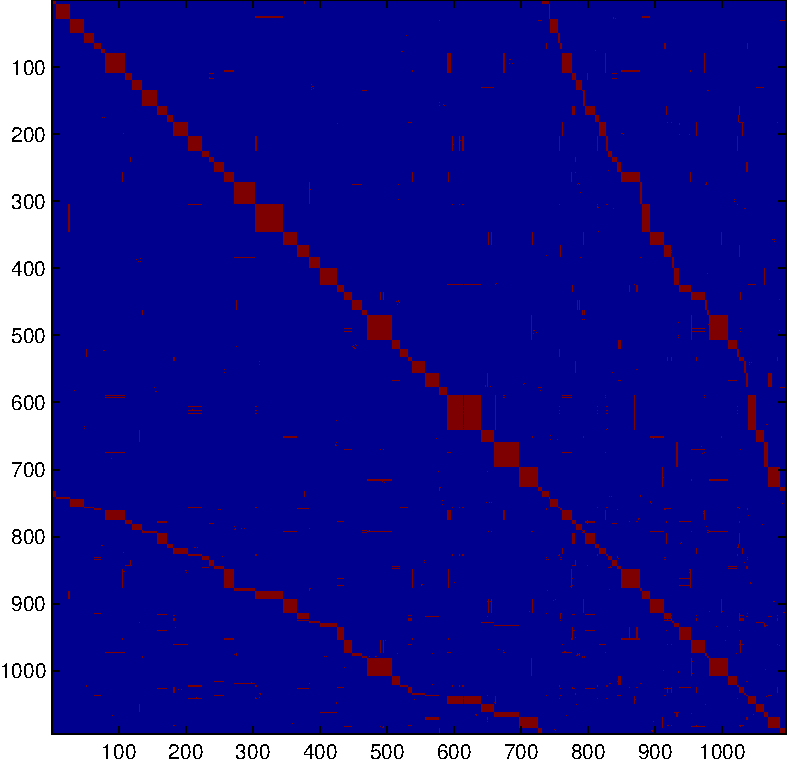
\includegraphics[width = \textwidth]{./img/adj6_3_s.pdf}
			\label{fig6_3_s_adj}
		\end{subfigure}
	\end{subfigure}

	\begin{subfigure}[c]{\textwidth}
		\centering
		\begin{subfigure}[c]{0.195\textwidth}
			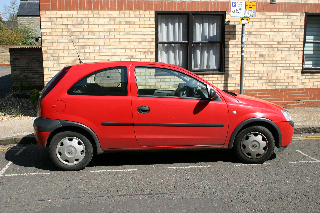
\includegraphics[width = \textwidth]{./img/7_8_s.png}
			\label{fig:7_8_s}

		\end{subfigure}
		\begin{subfigure}[c]{0.195\textwidth}
			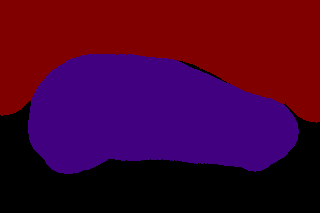
\includegraphics[width = \textwidth]{./img/7_8_s_GT.png}
			\label{fig:7_8_s_lab}
		\end{subfigure}
		\begin{subfigure}[c]{0.195\textwidth}
			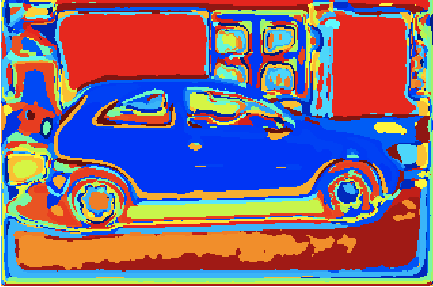
\includegraphics[width = \textwidth]{./img/7_8_s_map.png}
			\label{fig:7_8_s_map}
		\end{subfigure}
		\begin{subfigure}[]{0.195\textwidth}
			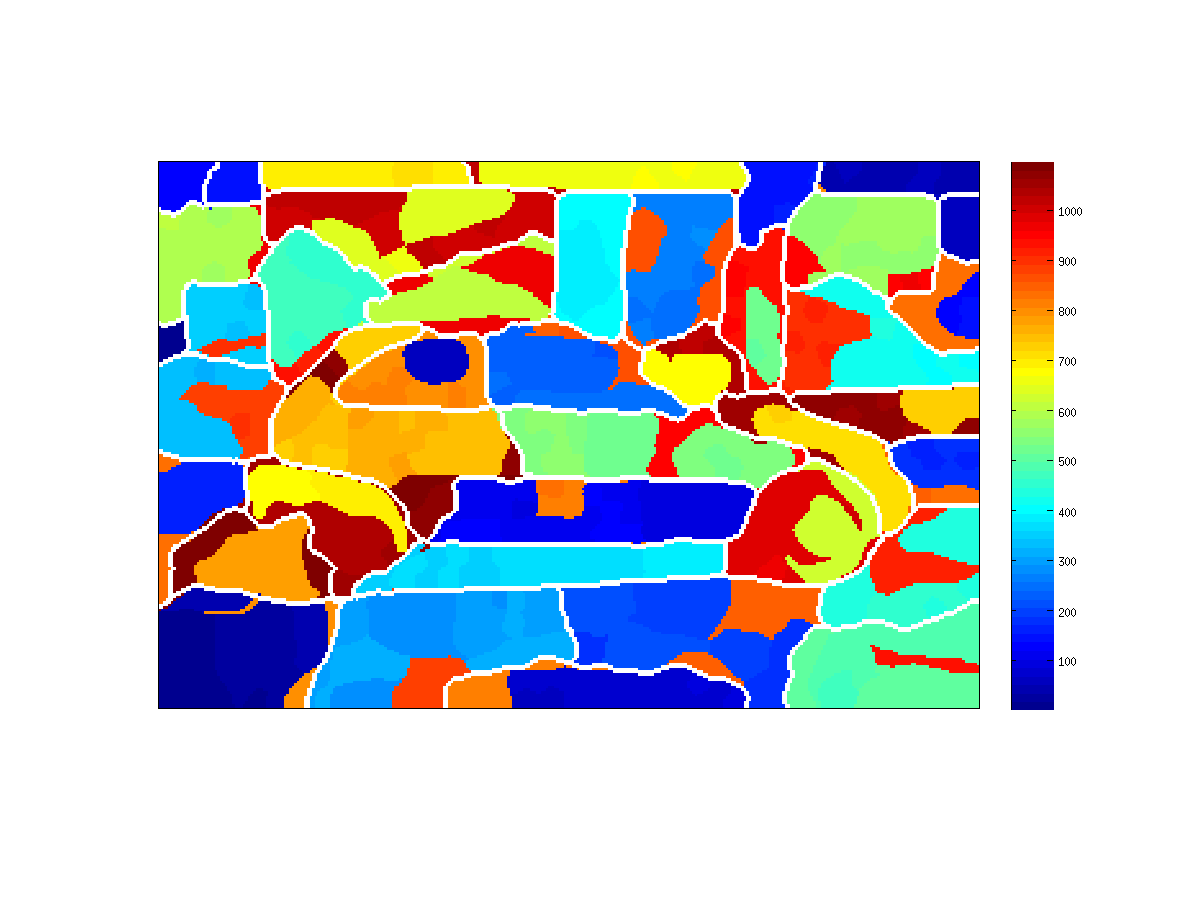
\includegraphics[width = \textwidth]{./img/su7_8_s.pdf}
			\label{fig:7_8_s_su}
		\end{subfigure}
		\begin{subfigure}[c]{0.195\textwidth}
			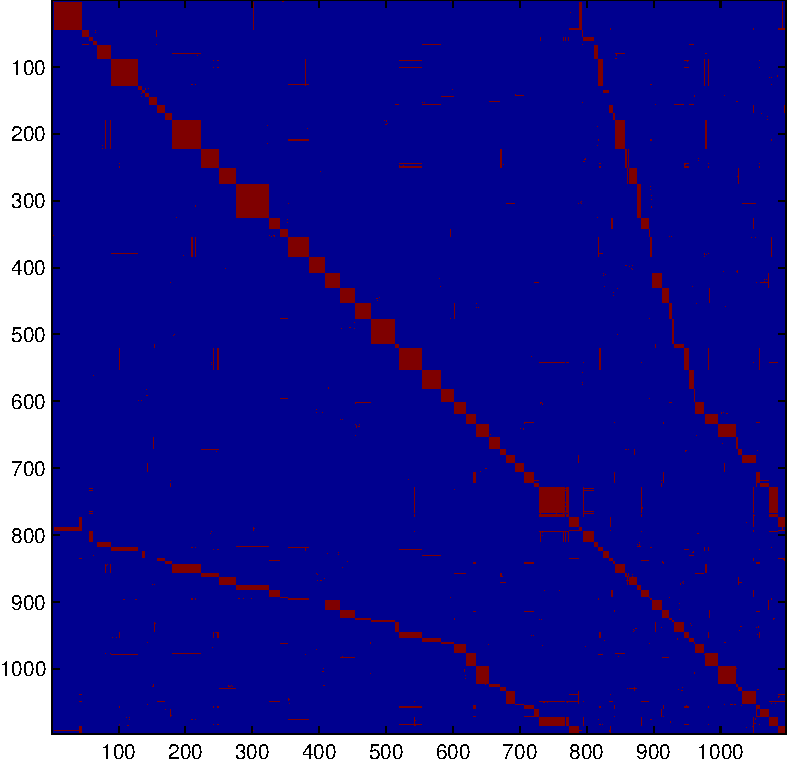
\includegraphics[width = \textwidth]{./img/adj7_8_s.pdf}
			\label{fig7_8_s_adj}
		\end{subfigure}
	\end{subfigure}

	
	\begin{subfigure}[t]{\textwidth}
		\centering
		\begin{subfigure}[t]{0.195\textwidth}
			\subcaption{original image}
		\end{subfigure}
		\begin{subfigure}[t]{0.195\textwidth}
			\subcaption{ground truth segmentation}
		\end{subfigure}
		\begin{subfigure}[t]{0.195\textwidth}
			\subcaption{visual words map}
		\end{subfigure}
		\begin{subfigure}[t]{0.195\textwidth}
			\subcaption{superpixel segmentation}
		\end{subfigure}
		\begin{subfigure}[t]{0.195\textwidth}
			\subcaption{superpixel adjacency matrix}
		\end{subfigure}
	\end{subfigure}

	\caption{}
\end{figure}
%------------------------------------------------------------------------------------------
\section{New Proposed Method}
\label{sec:New}
%------------------------------------------------------------------------------------------

\section{Conclusion}
\label{sec:Conclusion}
%------------------------------------------------------------------------------------------
\section{Plan of Activities}
\label{sec:Plan}

%------------------------------------------------------------------------------------------\bibliography{midway_report}
\bibliographystyle{plain}
\bibliography{midway_report}

\end{document}
